\section{Συμπεράσματα}\label{section:5-1-conclusions}

Συνοψίζοντας, μέσω της ανάπτυξης της πιλοτικής εφαρμογής Concordia γίνεται φανερό ότι είναι εφικτή η υλοποίηση μίας πλήρως αποκεντρωμένης κοινωνικής πλατφόρμας, η οποία να εκπληρώνει τον στόχο που τέθηκε στην \hyperref[section:1-4-thesis-goal]{ενότητα 1.4}, σύμφωνα με τον σχεδιασμό του \hyperref[chapter:3-application-design]{κεφαλαίου 3}.

Μέσω της αρχιτεκτονικής αποκέντρωσης των τριών επιπέδων της τεχνολογικής στοίβας (βλ. \hyperref[section:3-2-technology-stack]{ενότητα 3.2}), δημιουργείται ένα πολιτικά αποκεντρωμένος ψηφιακός χώρος, ο οποίος κατοχυρώνει την ελευθερία του λόγου των συμμετεχόντων και παρέχει παντοδύναμες αυθεντικές δημοκρατικές διαδικασίες.

Ωστόσο, θα πρέπει να επισημανθεί ότι η εφαρμογή χαρακτηρίζεται από ορισμένα μειονεκτήματα, τα οποία σχετίζονται, κυρίως, με την πρώιμη κατάσταση ανάπτυξης των επιλεγμένων τεχνολογιών:

\begin{itemize}
	\item Στο Application tier, μέσω της χρήσης του Ethereum, εισάγονται όλα εκείνα τα ζητήματα που συνοδεύουν επί του παρόντος το blockchain και τα smart contracts. Τα βασικότερα από αυτά είναι τα τέλη των συναλλαγών, η ανάγκη χρήσης επιπρόσθετων λογισμικών (π.χ. MetaMask) και η κλιμακοθετησιμότητά (scalability) των DApp. Σε γενικές γραμμές, το κλίμα στην παγκόσμια προγραμματιστική κοινότητα παραμένει αρκέτα πολωμένο ως προς το αν τελικά πλατφόρμες όπως το Ethereum θα μπορέσουν να ξεπεράσουν τα διάφορα προβλήματα και να ανταπεξέλθουν στις προσδοκίες.

	\begin{enumitemcenteredfigure}
		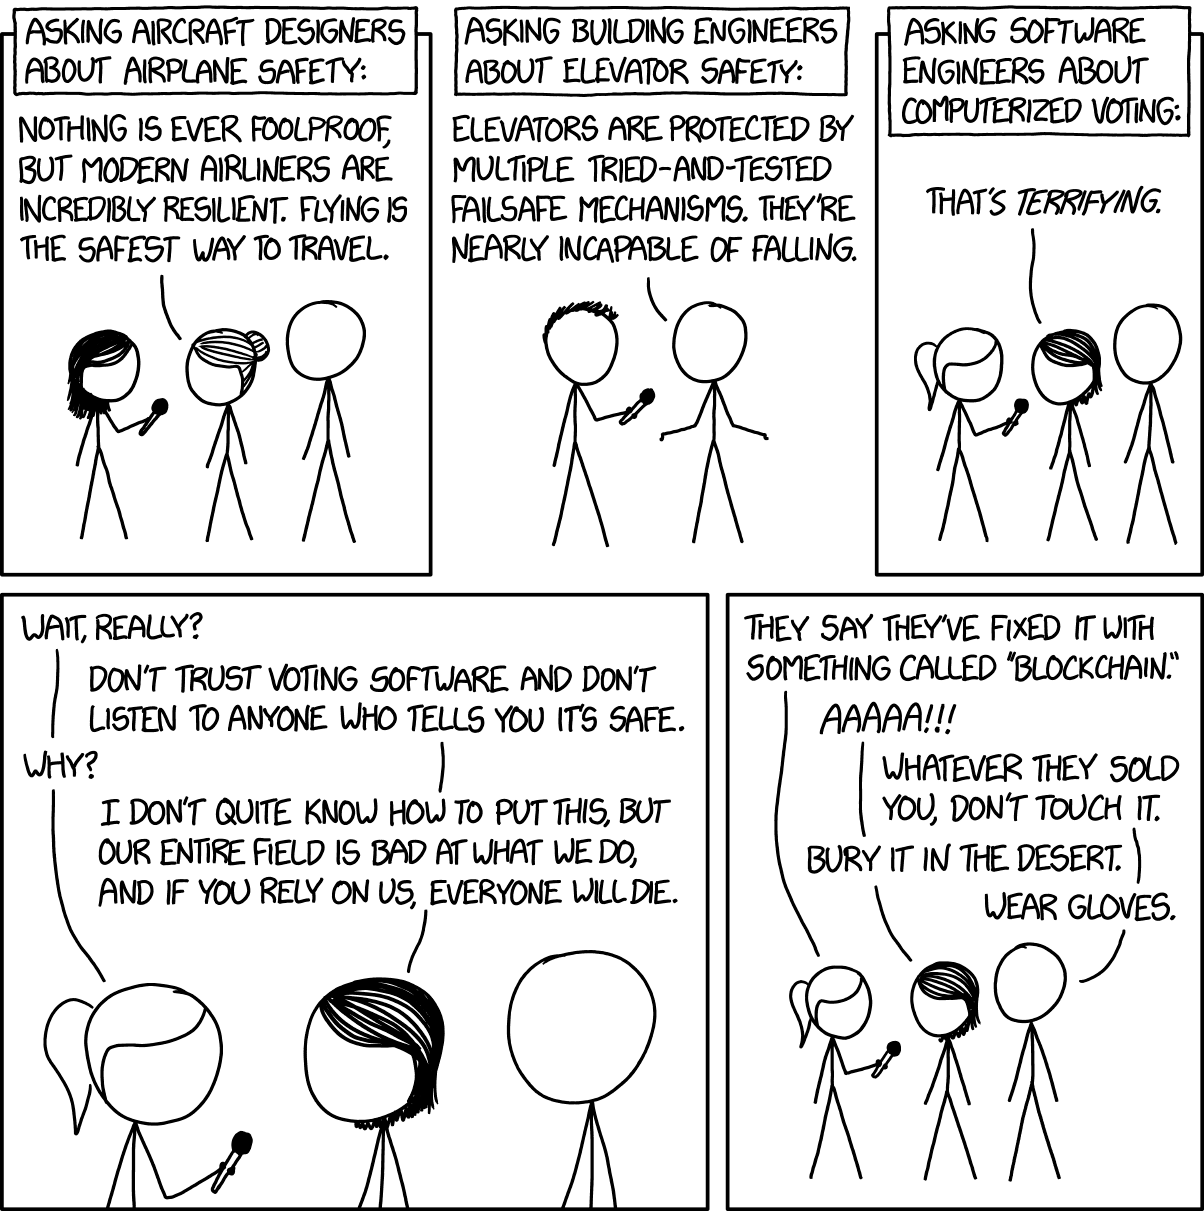
\includegraphics[width=.50\textwidth]{assets/figures/chapter-5/5.1.xkcd_2030_voting_software}
		\caption{\url{https://xkcd.com/2030/}}
	\end{enumitemcenteredfigure}

	\item Στο Data tier, το IPFS και η OrbitDB αποτελούν επίσης ιδιαίτερα καινοτόμα λογισμικά και δε θεωρούνται ακόμα production-ready. Αυτό έχει ως αποτέλεσμα να εισάγουν με τη σειρά τους διάφορα προβλήματα, τα οποία σχετίζονται κυρίως με την εύρεση των peers (το οποίο βασίζεται προσωρινά σε signalling servers\footnote{Βλ. και \url{https://github.com/libp2p/js-libp2p/issues/385}.}) και το replication των δεδομένων.
\end{itemize}

Τέλος, τονίζεται πως, παρ' όλες τις τρέχουσες δυσκολίες, οι προγραμματιστικές κοινότητες των παραπάνω τεχνολογιών εργάζονται αδιάκοπα για τη βελτίωση τους, ενώ παρόμοια εναλλακτικά project μπορούν ανά πάσα στιγμή να αντικαταστήσουν αυτά που επιλέχθηκαν στην τρέχουσα υλοποίηση.
